\documentclass[12pt,a4paper]{article}

% ── Encodage & langue ──────────────────────────────────────────────────────────
\usepackage[utf8]{inputenc}
\usepackage[T1]{fontenc}
\usepackage[french]{babel}

% ── Mise en page ───────────────────────────────────────────────────────────────
\usepackage[top=2.5cm, bottom=2.5cm, left=2.5cm, right=2.5cm]{geometry}
\usepackage{parskip}
\usepackage{setspace}
\usepackage[stable]{footmisc}
\onehalfspacing
\usepackage{pdflscape}

% ── Typographie ────────────────────────────────────────────────────────────────
\usepackage{lmodern}
\usepackage{microtype}

% ── Mathématiques ──────────────────────────────────────────────────────────────
\usepackage{amsmath, amssymb}

% ── Tableaux ───────────────────────────────────────────────────────────────────
\usepackage{booktabs}
\usepackage{tabularx}
\usepackage{array}
\usepackage{multirow}
\usepackage{longtable}

% ── Graphics ───────────────────────────────────────────────────────────────────
\usepackage{graphicx}
\graphicspath{{img/}{../img/}{../../img/}{../../../img/}{../../../../img/}}
% ── wrapfigure ─────────────────────────────────────────────────────────────────
\usepackage{wrapfig}
\usepackage{float}

% ── Code source ────────────────────────────────────────────────────────────────
\usepackage{listings}
\usepackage{xcolor}

\definecolor{codebg}{RGB}{245,245,245}
\definecolor{codeframe}{RGB}{200,200,200}
\definecolor{codecomment}{RGB}{100,100,100}
\definecolor{codestring}{RGB}{163,21,21}
\definecolor{codekeyword}{RGB}{0,0,255}

\lstset{
  backgroundcolor=\color{codebg},
  frame=single,
  rulecolor=\color{codeframe},
  basicstyle=\ttfamily\small,
  keywordstyle=\color{codekeyword}\bfseries,
  stringstyle=\color{codestring},
  commentstyle=\color{codecomment}\itshape,
  breaklines=true,
  showstringspaces=false,
  language=Python,
  literate=
    {é}{{\'{e}}}1 {è}{{\`{e}}}1 {ê}{{\^{e}}}1 {ë}{{\"e}}1
    {à}{{\`{a}}}1 {â}{{\^{a}}}1 {î}{{\^{i}}}1 {ô}{{\^{o}}}1
    {û}{{\^{u}}}1 {ù}{{\`{u}}}1 {ç}{{\c{c}}}1 {œ}{{\oe}}1
}

% ── Boîtes colorées (pour les remarques / avertissements) ──────────────────────
\usepackage{mdframed}

\newmdenv[
  backgroundcolor=blue!5,
  linecolor=blue!50!black,
  linewidth=1pt,
  innerleftmargin=10pt,
  innerrightmargin=10pt,
  innertopmargin=6pt,
  innerbottommargin=6pt,
  skipabove=8pt,
  skipbelow=8pt
]{remarque}

\newmdenv[
  backgroundcolor=orange!10,
  linecolor=orange!70!black,
  linewidth=1pt,
  innerleftmargin=10pt,
  innerrightmargin=10pt,
  innertopmargin=6pt,
  innerbottommargin=6pt,
  skipabove=8pt,
  skipbelow=8pt
]{avertissement}

% ── Hyperliens ─────────────────────────────────────────────────────────────────
\usepackage[colorlinks=true, linkcolor=blue!70!black, urlcolor=blue!70!black]{hyperref}
\usepackage{bookmark}

% ── En-têtes / pieds de page ───────────────────────────────────────────────────
\usepackage{fancyhdr}
\setlength{\headheight}{14.2pt}
\addtolength{\topmargin}{-2.2pt}
\pagestyle{fancy}
\fancyhf{}
\lhead{\small Compte-rendu technique --- Étape 2}
\rhead{\small LARROUX Logan}
\cfoot{\thepage}
\renewcommand{\headrulewidth}{0.4pt}

% ══════════════════════════════════════════════════════════════════════════════
\begin{document}

% ── Page de titre ──────────────────────────────────────────────────────────────
\begin{titlepage}
  \centering

  \vspace{3cm}

  {\fontsize{20}{22}\selectfont\bfseries
    COMPTE-RENDU TECHNIQUE\\
    Analyse de conversations patient-thérapeute\\
    sur la santé mentale\par}
  {\color{blue!70!black}\rule{0.5\textwidth}{1.5pt}\par}
  \vspace{0.5cm}

  {\large\bfseries Auteur: LARROUX Logan \\
                  Encadrante : Lynda Tamine-Lechani\par}

  {\normalsize\itshape
    Équipe :\\[0.3em]
    Ulysse Chasseigne, Idir Yahiaoui, Bantsoukissa Laure,\\
    Cruz Fernandes Diogo, Emin Belkheir, Esso-Y-N Trésor PANA,\\
    Logan Larroux, Yvan Sellier, Victor Blanquart--Blanchet, Lucas Da Silva\par}

  \vspace{0.8cm}
  {\fontsize{14}{18}\selectfont\today\par}

  \vspace{1cm}
  \begin{tabular}[t]{c}
    \centering
    
\includegraphics[height=1.5cm]{universite-de-toulouse-logo.png}
    \hspace{10px}
    {
\includegraphics[height=1.5cm]{IRIT_logo.png}}
    \hspace{10px}
    \raisebox{0.70cm}{\normalsize [Info5.BE-SHS]\par}
  \end{tabular}

  \vfill

  {\color{blue!70!black}\rule{\textwidth}{0.4pt}\par}
  \vspace{0.4cm}
  {\small Données : \href{https://www.kaggle.com/datasets/thedevastator/nlp-mental-health-conversations}{Kaggle --- NLP Mental Health Conversations}\par}
  \vspace{0.2cm}
  {\small Code : \href{https://github.com/cypnet/Analyse-de-conversations-sur-la-sant-mentale/tree/main/notebooks/LOGAN}{GitHub --- branche Logan}\par}
  \vspace{0.5cm}
\end{titlepage}

% ── Table des matières ─────────────────────────────────────────────────────────
\tableofcontents
\newpage

% ==============================================================================
\section{Contexte et organisation}
% ==============================================================================

L'étape 2 a divisé le groupe 1 en deux sous-groupes travaillant en parallèle sur le même jeu de données d'entraînement (\texttt{combined\_data.csv}, \textit{Sentiment Analysis for Mental Health} sur Kaggle), avec pour objectif commun d'annoter automatiquement le dataset principal \texttt{train.csv} en vue de sa transmission au Groupe 2.

\begin{center}
\begin{tabular}{lll}
\toprule
\textbf{Sous-groupe} & \textbf{Méthode} & \textbf{Membres} \\
\midrule
Supervisé    & Naive Bayes (BoW + TF-IDF) & \\
             & + Logistic Regression (TF-IDF) &  \\
             & + LinearSVC (BoW + TF-IDF) & Diogo, Ulysse, Logan \\
\midrule
Non-supervisé & K-Means (Word2Vec + TF-IDF)                               & Emin, Victor \\
\bottomrule
\end{tabular}
\end{center}

Le pipeline commun aux deux sous-groupes comprend : nettoyage du texte, tokenisation (NLTK + Porter Stemmer), et vectorisation (BoW, TF-IDF, Word2Vec). Le split des données est identique pour les deux : \textbf{60\,\% train / 20\,\% validation / 20\,\% test}, avec stratification sur les classes.

% ------------------------------------------------------------------------------
\subsection{Différence entre méthode supervisée et non-supervisée}
% ------------------------------------------------------------------------------

\textbf{Une méthode supervisée} apprend à partir d'\textbf{exemples déjà étiquetés}. Pour chaque entrée, on connaît la bonne réponse pendant l'entraînement~; le modèle apprend donc à associer des entrées à des sorties connues.\\
\textit{Exemple} : classer des e-mails en spam / non-spam, prédire un prix, détecter une maladie à partir de symptômes.

\textbf{Une méthode non-supervisée}, quant à elle, apprend à partir de \textbf{données non étiquetées}. Il n'existe pas de bonne réponse fournie au préalable~; le but est de découvrir des structures cachées, des groupes ou des patterns dans les données.\\
\textit{Exemple} : regrouper des clients en segments, détecter des anomalies, réduire la dimension des données.

En résumé :
\begin{itemize}
  \item Supervisée $\rightarrow$ on connaît la réponse attendue.
  \item Non-supervisée $\rightarrow$ on ne connaît pas la réponse, on cherche des structures.
\end{itemize}

% ------------------------------------------------------------------------------
\subsection{Métriques d'évaluation utilisées}
% ------------------------------------------------------------------------------

Afin de comparer les modèles et sélectionner le meilleur pour annoter \texttt{train.csv}, nous distinguons trois catégories de métriques selon leur domaine d'application.

% ------------------------------------------------------------------------------
\subsubsection{Métriques communes aux deux méthodes}
% ------------------------------------------------------------------------------

Ces deux métriques s'appliquent aussi bien à la méthode supervisée qu'à la méthode non-supervisée (après association des clusters aux labels pour cette dernière), ce qui en fait les seuls indicateurs permettant une \textbf{comparaison directe} entre les deux approches.

\paragraph{Accuracy}

Pourcentage de sentiments correctement prédits :

\[
  \text{Accuracy} = \frac{\text{Nb. de bonnes prédictions}}{\text{Nb. total d'exemples}}
\]

\paragraph{Matrice de confusion}

Permet de visualiser les prédictions par rapport aux vraies classes. Les lignes représentent les vraies classes, les colonnes les classes prédites. Elle révèle les erreurs systématiques du modèle~: quelles classes sont confondues entre elles, et dans quelle direction.

% ------------------------------------------------------------------------------
\subsubsection{Métriques propres à la méthode supervisée}
% ------------------------------------------------------------------------------

Ces métriques nécessitent de connaître les vrais labels pour chaque exemple, ce qui est possible en apprentissage supervisé mais pas directement applicable au clustering non-supervisé.

\paragraph{MSE (Mean Squared Error)}

Erreur moyenne au carré entre la vraie valeur et la valeur prédite :

\[
  \text{MSE} = \frac{1}{n}\sum_{i=1}^{n}(y_i - \hat{y}_i)^2
\]

\paragraph{R² (Coefficient de détermination)}

Mesure la proportion de variance des données expliquée par le modèle :

\[
  R^2 = 1 - \frac{\text{Erreur modèle}}{\text{Erreur moyenne}}
\]

\begin{avertissement}
\textbf{Attention --- MSE et R² sont des métriques de régression.} Elles supposent qu'il existe un ordre et une distance numérique significative entre les valeurs prédites et les valeurs réelles. Or nos labels sont nominaux (\texttt{Depression}, \texttt{Anxiety}, \texttt{Normal}\ldots) encodés arbitrairement en entiers~: la "distance" entre deux classes n'a aucun sens clinique ni mathématique. Ces deux métriques ne sont donc \textbf{pas des indicateurs fiables} pour ce problème et ne doivent pas être utilisées comme critères de décision. L'accuracy et le F1-score sont à privilégier.
\end{avertissement}

\paragraph{Precision, Recall et F1-score}

Ces trois métriques issues du classification report permettent d'évaluer les performances \textbf{classe par classe}, ce qui est essentiel ici en raison du fort déséquilibre entre les 7 catégories de sentiments.

\begin{itemize}
  \item \textbf{Precision} --- parmi les prédictions positives, combien sont vraiment positives ?
  \[
    \text{Precision} = \frac{TP}{TP + FP}
  \]
  \item \textbf{Recall} --- parmi les vrais positifs, combien ont été retrouvés ?
  \[
    \text{Recall} = \frac{TP}{TP + FN}
  \]
  \item \textbf{F1-score} --- compromis entre precision et recall, particulièrement utile sur des classes déséquilibrées :
  \[
    F1 = 2 \times \frac{\text{Precision} \times \text{Recall}}{\text{Precision} + \text{Recall}}
  \]
\end{itemize}

Avec : TP = vrai positif, TN = vrai négatif, FP = faux positif, FN = faux négatif.

\begin{remarque}
Pour comparer les méthodes supervisées entre elles (NB vs LR), nous privilégions le \textbf{F1-score macro} (moyenne non pondérée sur les classes) plutôt que le F1 \textit{weighted}, afin de ne pas masquer les mauvaises performances sur les classes minoritaires (\textit{Stress}, \textit{Personality disorder}).
\end{remarque}

% ------------------------------------------------------------------------------
\subsubsection{Métriques propres à la méthode non-supervisée}
% ------------------------------------------------------------------------------

Ces métriques sont spécifiques au clustering~: elles évaluent la qualité des groupes formés \textbf{sans faire référence aux vrais labels} pendant l'entraînement, ce qui les rend non comparables directement avec les métriques supervisées.

\paragraph{Purity globale}

Mesure la cohérence interne des clusters~: pour chaque cluster, on retient uniquement le label majoritaire parmi ses membres.

\[
  \text{Purity} = \frac{1}{N}\sum_k \max_j |C_k \cap L_j|
\]

Avec $N$ le nombre total d'exemples, $C_k$ le cluster $k$ et $L_j$ la classe réelle $j$.

\begin{remarque}
Plus la Purity est proche de 1, meilleur est le regroupement. Attention~: si chaque point forme son propre cluster, la purity vaut 1 --- cette mesure peut donc être trompeuse si utilisée seule.
\end{remarque}

\paragraph{ARI (Adjusted Rand Index)}

Mesure la similarité entre les vrais labels et les clusters trouvés, en corrigeant le score pour tenir compte du hasard. Sa valeur est comprise entre $-1$ (pire qu'aléatoire) et $1$ (clustering parfait). Contrairement à la Purity, l'ARI \textbf{pénalise un trop grand nombre de clusters} et les mauvais regroupements, ce qui en fait un indicateur plus robuste.

% ------------------------------------------------------------------------------
\subsubsection{Tableau récapitulatif}
% ------------------------------------------------------------------------------

\begin{center}
\renewcommand{\arraystretch}{1.2}
\begin{tabular}{llcc}
\toprule
\textbf{Catégorie} & \textbf{Mesure} & \textbf{Supervisée} & \textbf{Non-supervisée} \\
\midrule
\multirow{2}{*}{Communes}
  & Accuracy          & Oui & Oui (après mapping) \\
  & Matrice confusion & Oui & Oui \\
\midrule
\multirow{5}{*}{Supervisée uniquement}
  & MSE               & Oui & Non \\
  & R²                & Oui & Non \\
  & Precision         & Oui & Non \\
  & Recall            & Oui & Non \\
  & F1-score          & Oui & Non \\
\midrule
\multirow{2}{*}{Non-supervisée uniquement}
  & Purity            & Non & Oui \\
  & ARI               & Non & Oui \\
\bottomrule
\end{tabular}
\end{center}

\pagebreak

% ==============================================================================
\section{Résultats par membre}
% ==============================================================================

% ------------------------------------------------------------------------------
\subsection{Méthode supervisée --- Naive Bayes et Logistic Regression}
% ------------------------------------------------------------------------------

\subsubsection*{Qu'est-ce que Naive Bayes ?}

Naive Bayes répond à la question : \textbf{«~Étant donné les mots de ce texte, quelle est la catégorie la plus probable~?~»}

C'est un classificateur probabiliste~: plutôt que de tracer une frontière entre les classes comme le ferait un SVM, il \textbf{calcule une probabilité} pour chaque classe et retourne celle qui est la plus élevée, en s'appuyant sur le théorème de Bayes~:

\[
  P(\text{classe} \mid \text{mots}) \propto P(\text{classe}) \times \prod_i P(\text{mot}_i \mid \text{classe})
\]

Le modèle fait une hypothèse simplificatrice~: chaque mot est supposé \textbf{indépendant} des autres. Cette simplification rend l'algorithme très rapide à entraîner et étonnamment efficace sur les textes malgré son aspect «~naïf~».

\subsubsection*{Qu'est-ce que la Logistic Regression ?}

La Régression Logistique répond à la question : \textbf{«~Étant donné ce vecteur TF-IDF, à quelle classe ce texte appartient-il le plus probablement~?~»}

Contrairement à Naive Bayes qui calcule des probabilités indépendamment mot par mot, la Régression Logistique \textbf{apprend un poids pour chaque feature} (ici chaque $n$-gram TF-IDF) et combine ces poids pour produire un score par classe.

\begin{center}
\renewcommand{\arraystretch}{1.2}
\begin{tabular}{lll}
\toprule
 & \textbf{Naive Bayes} & \textbf{Logistic Regression} \\
\midrule
Hypothèse               & Mots indépendants            & Aucune hypothèse sur les features \\
Frontière               & Probabiliste naïve           & Frontière de décision optimisée \\
Classes déséquilibrées  & Biais vers la classe majoritaire & Géré via \texttt{class\_weight='balanced'} \\
Corrélations entre mots & Ignorées                     & Prises en compte implicitement \\
\bottomrule
\end{tabular}
\end{center}

Le paramètre clé de la LR est \textbf{\texttt{C}} (inverse de la régularisation)~: un \texttt{C} petit entraîne une régularisation forte (modèle simple, évite l'overfitting) ; un \texttt{C} grand entraîne une régularisation faible (modèle plus complexe, peut overfit).

\subsubsection*{Qu'est-ce que LinearSVC ?}

Le LinearSVC répond à la question~: \textbf{«~Quelle est la frontière optimale qui sépare le mieux les classes~?~»}

Contrairement à la Régression Logistique qui estime des probabilités, le LinearSVC cherche un \textbf{hyperplan} (une droite en 2D, un plan en 3D, généralisé en $N$ dimensions) qui sépare les classes en \textbf{maximisant la marge}, c'est-à-dire la distance entre la frontière et les points les plus proches de chaque classe. Ces points les plus proches sont les \textbf{vecteurs de support}~: ils sont les seuls à définir la frontière, tous les autres exemples n'ont aucune influence.

La frontière est linéaire, ce qui est parfaitement adapté aux vecteurs TF-IDF déjà en haute dimension. \textbf{En haute dimension, les classes sont souvent linéairement séparables même si elles ne le seraient pas en 2D.}

\begin{center}
\renewcommand{\arraystretch}{1.2}
\begin{tabular}{lccc}
\toprule
 & \textbf{Naive Bayes} & \textbf{Logistic Regression} & \textbf{LinearSVC} \\
\midrule
Approche        & Probabiliste        & Probabiliste                  & \textbf{Géométrique} \\
Apprend         & $P(\text{classe}|\text{mots})$ & Poids par feature & Frontière à marge max \\
Sortie          & Probabilité         & Probabilité                   & \textbf{Score de décision} \\
Déséquilibre    & Sensible            & Géré via \texttt{class\_weight} & Géré via \texttt{class\_weight} \\
Vitesse         & Très rapide         & Rapide                        & Très rapide (haute dim.) \\
Atout principal & Simplicité          & Calibration                   & \textbf{Marge max} \\
                &                     &                               & $\rightarrow$\textbf{meilleure généralisation} \\
\bottomrule
\end{tabular}
\end{center}

\begin{remarque}
LinearSVC est souvent le modèle le plus performant sur des tâches de classification de texte TF-IDF, car il est nativement conçu pour les espaces de haute dimension et les données creuses (\textit{sparse}), ce qui correspond exactement aux vecteurs TF-IDF.
\end{remarque}

\pagebreak
% ------------------------------------------------------------------------------
\subsubsection{Diogo et Ulysse --- Naive Bayes BoW et TF-IDF}
% ------------------------------------------------------------------------------

Diogo et Ulysse ont produit les résultats de référence pour la méthode supervisée.

\textbf{Tuning de l'hyperparamètre \texttt{alpha} (lissage de Laplace)~:}
\begin{itemize}
  \item Valeurs testées : \texttt{[0.001, 0.01, 0.05, 0.1, 0.5, 1.0, 2.0, 5.0]}
  \item Meilleur alpha BoW : \textbf{0.1} (accuracy validation : 0.6606)
  \item Meilleur alpha TF-IDF : \textbf{0.05} (accuracy validation : 0.6761)
\end{itemize}

\textbf{Résultats sur l'ensemble test~:}

\begin{center}
\begin{tabular}{ll}
\toprule
\textbf{Modèle} & \textbf{Accuracy test} \\
\midrule
Naive Bayes + BoW    & \textbf{0.6666} \\
Naive Bayes + TF-IDF & \textbf{0.6875} \\
\bottomrule
\end{tabular}
\end{center}

\textbf{Classification report (NB + BoW)~:}

\begin{center}
\begin{tabular}{lccc}
\toprule
\textbf{Classe} & \textbf{Precision} & \textbf{Recall} & \textbf{F1-score} \\
\midrule
Anxiety              & 0.68 & 0.73 & 0.71 \\
Bipolar              & 0.60 & 0.76 & 0.68 \\
Depression           & 0.57 & 0.61 & 0.59 \\
Normal               & 0.92 & 0.70 & 0.80 \\
Personality disorder & 0.50 & 0.56 & 0.53 \\
Stress               & 0.52 & 0.43 & 0.47 \\
Suicidal             & 0.60 & 0.72 & 0.65 \\
\bottomrule
\end{tabular}
\end{center}

\begin{figure}[H]
  \centering
  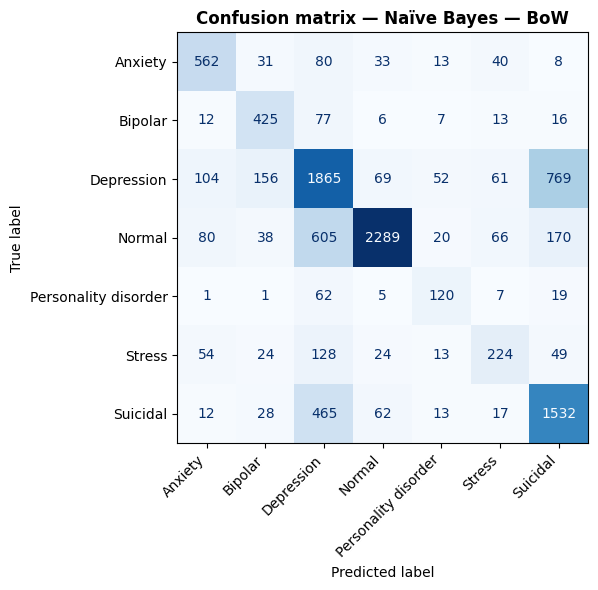
\includegraphics[width=0.75\textwidth]{matriceConfusion_NB_BoW_Diogo_Ulysse.png}
  \caption{Matrice de confusion --- NB + BoW (Diogo et Ulysse)}
\end{figure}

\textbf{Classification report (NB + TF-IDF)~:}

\begin{center}
\begin{tabular}{lccc}
\toprule
\textbf{Classe} & \textbf{Precision} & \textbf{Recall} & \textbf{F1-score} \\
\midrule
Anxiety              & 0.76 & 0.71 & 0.73 \\
Bipolar              & 0.82 & 0.58 & 0.68 \\
Depression           & 0.54 & 0.77 & 0.63 \\
Normal               & 0.90 & 0.77 & 0.83 \\
Personality disorder & 0.97 & 0.29 & 0.45 \\
Stress               & 0.83 & 0.27 & 0.41 \\
Suicidal             & 0.65 & 0.60 & 0.62 \\
\bottomrule
\end{tabular}
\end{center}

\begin{figure}[H]
  \centering
  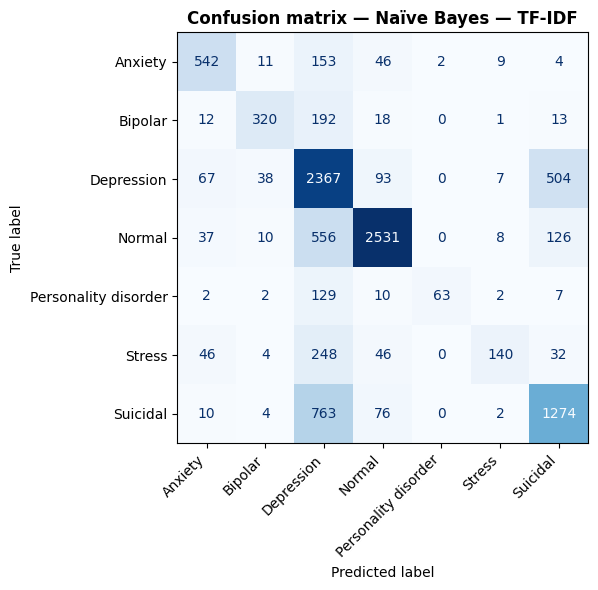
\includegraphics[width=0.75\textwidth]{matriceConfusion_NB_TF-IDF_Diogo_Ulysse.png}
  \caption{Matrice de confusion --- NB + TF-IDF (Diogo et Ulysse)}
\end{figure}

\begin{remarque}
TF-IDF est meilleur sur les deux classes les plus représentées (\textit{Normal} et \textit{Depression}), ce qui tire son accuracy globale vers le haut. Mais sur les 5 autres classes, \textbf{BoW gagne à chaque fois}, parfois très largement : \textit{Stress} (43\,\% vs 27\,\% de recall) ou \textit{Bipolar} (76\,\% vs 58\,\% de recall).

\textbf{Pourquoi ?} TF-IDF pénalise les mots fréquents. C'est utile pour séparer \textit{Normal} de \textit{Depression}, mais pour les classes rares (\textit{Stress}, \textit{Personality disorder}), les mots caractéristiques sont précisément des mots fréquents dans le corpus global (\textit{overwhelmed}, \textit{pressure}, \textit{relationship}\ldots). TF-IDF les «~dépouille~» de leur signal. Le cas de \textit{Personality disorder} est frappant~: \textbf{precision 0.97 mais recall 0.29} --- le modèle est très sûr quand il prédit cette classe, mais il rate 71\,\% des vrais cas.
\end{remarque}

\pagebreak
% ------------------------------------------------------------------------------
\subsubsection{Logan --- Naive Bayes + Logistic Regression}
% ------------------------------------------------------------------------------

Logan a produit le notebook de base structurant le travail commun. Sa contribution individuelle principale est l'implémentation d'une \textbf{Régression Logistique} (LR + TF-IDF optimisé), identifiée comme «~version extra-performante~».

\textbf{Paramétrage TF-IDF amélioré~:}
\begin{lstlisting}
tfidf_vectorizer = TfidfVectorizer(
    ngram_range=(1, 3),   # unigrammes, bigrammes et trigrammes
    max_features=50000,   # limite aux 50k features les plus utiles
    sublinear_tf=True,    # log(tf) au lieu de tf
    min_df=2,             # ignore les mots < 2 documents
    max_df=0.95           # ignore les mots > 95% des documents
)
\end{lstlisting}

\textbf{Tuning de l'hyperparamètre \texttt{alpha} (Naive Bayes)~:}
\begin{itemize}
  \item Valeurs testées : \texttt{[0.001, 0.005, 0.01, 0.03, 0.05, 0.07, 0.1]}
  \item Meilleur alpha BoW : \textbf{0.1} (accuracy : 0.6606)
  \item Meilleur alpha TF-IDF : \textbf{0.07} (accuracy : 0.6816)
\end{itemize}

\textbf{Tuning de l'hyperparamètre \texttt{C} (Logistic Regression)~:}
\begin{itemize}
  \item Valeurs testées : \texttt{[0.01, 0.05, 0.1, 0.3, 0.5, 1.0, 3.0, 5.0, 10.0]}
  \item Meilleur C : \textbf{3.0} (accuracy validation : 0.7457)
\end{itemize}

\textbf{Résultats comparés sur l'ensemble test~:}

\begin{center}
\begin{tabular}{ll}
\toprule
\textbf{Modèle} & \textbf{Accuracy test} \\
\midrule
Naive Bayes + BoW            & 0.6666 \\
Naive Bayes + TF-IDF         & 0.6927 \\
Logistic Regression + TF-IDF & \textbf{0.7532} \\
\bottomrule
\end{tabular}
\end{center}

\textbf{Comparaison F1-score NB + TF-IDF vs LR + TF-IDF~:}

\begin{center}
\begin{tabular}{lccc}
\toprule
\textbf{Classe} & \textbf{F1 NB TF-IDF} & \textbf{F1 LR TF-IDF} & \textbf{Évolution} \\
\midrule
Anxiety              & 0.73 & 0.80 & $+0.07$ \\
Bipolar              & 0.67 & 0.79 & $+0.16$ \\
Depression           & 0.63 & 0.69 & $+0.06$ \\
Normal               & 0.85 & 0.90 & $+0.15$ \\
Personality disorder & 0.40 & 0.66 & $\mathbf{+0.26}$ \\
Stress               & 0.37 & 0.57 & $\mathbf{+0.20}$ \\
Suicidal             & 0.63 & 0.64 & $+0.01$ \\
\bottomrule
\end{tabular}
\end{center}

\begin{figure}[H]
  \centering
  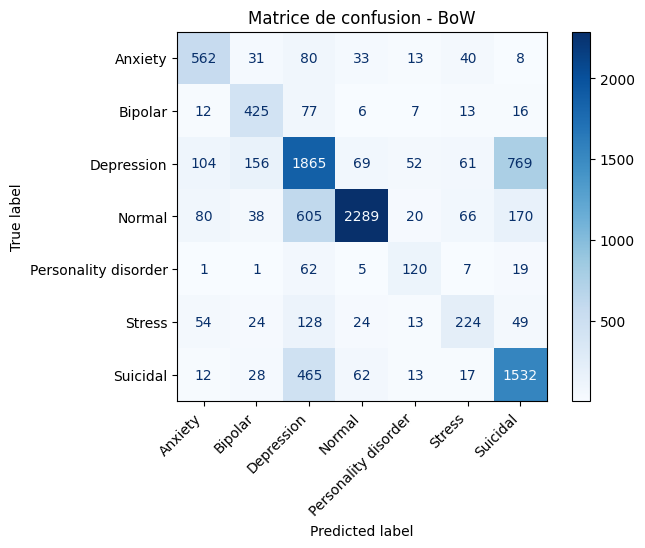
\includegraphics[width=0.75\textwidth]{matriceConfusion_NB_BoW_LOGAN.png}
  \caption{Matrice de confusion --- NB + BoW (Logan)}
\end{figure}

\begin{figure}[H]
  \centering
  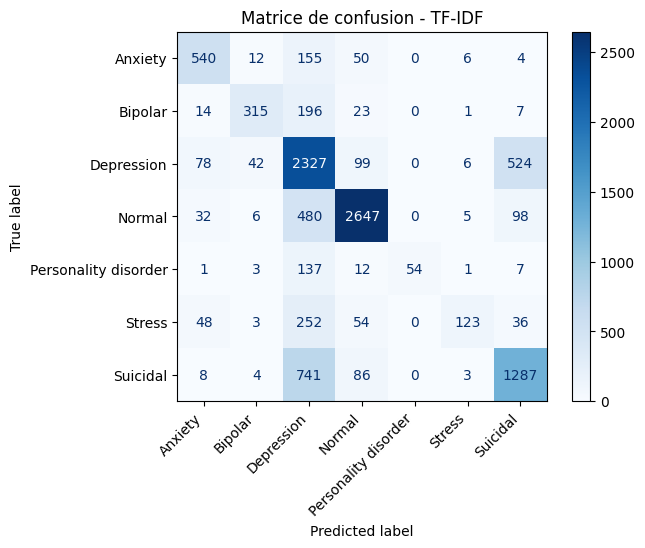
\includegraphics[width=0.75\textwidth]{matriceConfusion_NB_TF-IDF_Logan.png}
  \caption{Matrice de confusion --- NB + TF-IDF (Logan)}
\end{figure}

\begin{figure}[H]
  \centering
  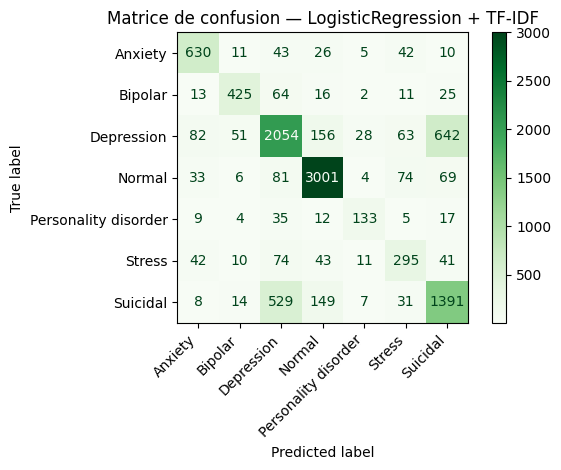
\includegraphics[width=0.75\textwidth]{matriceConfusion_LR_TF-IDF_Logan.png}
  \caption{Matrice de confusion --- LR + TF-IDF (Logan)}
\end{figure}

\begin{remarque}
La Logistic Regression améliore le F1-score sur \textbf{toutes les classes}, en particulier \textit{Personality disorder} ($+0.26$) et \textit{Stress} ($+0.20$) grâce au paramètre \texttt{class\_weight='balanced'} qui compense le déséquilibre du dataset.
\end{remarque}

\begin{avertissement}
\textbf{Problème critique --- classe \textit{Suicidal}~:} sur 2\,129 vrais cas \textit{Suicidal}, 1\,391 sont correctement classés \textbf{mais 529 sont prédits \textit{Depression}}. Confondre \textit{Suicidal} avec \textit{Depression} peut avoir des conséquences réelles dans un contexte médical. Ce problème est commun à toutes les approches testées.
\end{avertissement}

\pagebreak
% ------------------------------------------------------------------------------
\subsubsection{Diogo --- LinearSVC + BoW et TF-IDF}
% ------------------------------------------------------------------------------

Après l'implémentation de Naive Bayes et Logistic Regression, Diogo a exploré le \textbf{LinearSVC} (\textit{Linear Support Vector Classifier}), une méthode géométriquement très différente des approches probabilistes précédentes.

\textbf{Tuning de l'hyperparamètre \texttt{C}~:}
\begin{itemize}
  \item Valeurs testées : \texttt{[0.01, 0.1, 1.0]}
  \item Meilleur C BoW : \textbf{0.1} (accuracy : 0.7309)
  \item Meilleur C TF-IDF : \textbf{1.0} (accuracy : 0.7386)
\end{itemize}

\begin{remarque}
Avec seulement 3 valeurs testées, le temps de traitement atteint déjà \textbf{8 minutes}. Une stratégie d'optimisation \textit{coarse-to-fine} est envisageable~: une \textit{coarse search} sur une large plage (ex.~: 0.001, 0.01, 0.1, 1, 10, 100) pour repérer la bonne zone, puis une \textit{fine search} plus précise autour des meilleures valeurs trouvées.
\end{remarque}

\textbf{Classification report (LinearSVC + BoW)~:}

\begin{center}
\begin{tabular}{lccc}
\toprule
\textbf{Classe} & \textbf{Precision} & \textbf{Recall} & \textbf{F1-score} \\
\midrule
Anxiety              & 0.77 & 0.73 & 0.75 \\
Bipolar              & 0.79 & 0.73 & 0.76 \\
Depression           & 0.71 & 0.65 & 0.68 \\
Normal               & 0.84 & 0.95 & 0.89 \\
Personality disorder & 0.68 & 0.59 & 0.63 \\
Stress               & 0.52 & 0.46 & 0.49 \\
Suicidal             & 0.63 & 0.63 & 0.63 \\
\bottomrule
\end{tabular}
\end{center}

\begin{figure}[H]
  \centering
  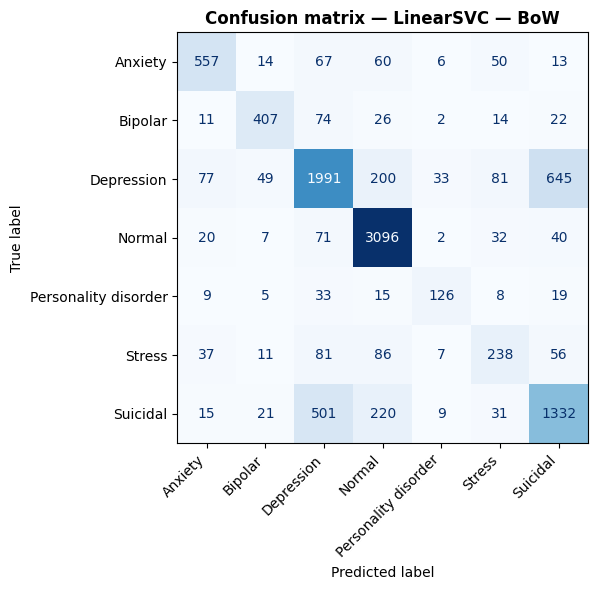
\includegraphics[width=0.75\textwidth]{matriceConfusion_LSVC_CBOW.png}
  \caption{Matrice de confusion --- LinearSVC + BoW (Diogo)}
\end{figure}

\textbf{Classification report (LinearSVC + TF-IDF)~:}

\begin{center}
\begin{tabular}{lccc}
\toprule
\textbf{Classe} & \textbf{Precision} & \textbf{Recall} & \textbf{F1-score} \\
\midrule
Anxiety              & 0.81 & 0.79 & 0.80 \\
Bipolar              & 0.86 & 0.71 & 0.78 \\
Depression           & 0.68 & 0.70 & 0.69 \\
Normal               & 0.85 & 0.94 & 0.89 \\
Personality disorder & 0.86 & 0.56 & 0.68 \\
Stress               & 0.68 & 0.46 & 0.55 \\
Suicidal             & 0.63 & 0.61 & 0.62 \\
\bottomrule
\end{tabular}
\end{center}

\begin{figure}[H]
  \centering
  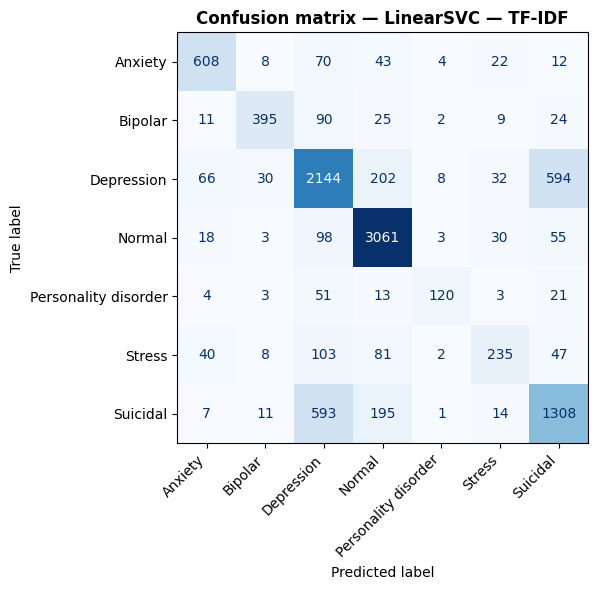
\includegraphics[width=0.75\textwidth]{matriceConfusion_LSVC_TFIDF.png}
  \caption{Matrice de confusion --- LinearSVC + TF-IDF (Diogo)}
\end{figure}

\textbf{Analyse détaillée des confusions~:}

\begin{center}
\renewcommand{\arraystretch}{1.2}
\begin{tabular}{lcc}
\toprule
\textbf{Modèle} & \textbf{Vrais \textit{Suicidal}} & \textbf{Vrais \textit{Depression}} \\
                & $\to$ \textbf{prédits \textit{Depression}} & $\to$ \textbf{prédits \textit{Suicidal}} \\
\midrule
LinearSVC TF-IDF & 593 & 594 \\
LinearSVC BoW    & 501 & 645 \\
\bottomrule
\end{tabular}
\end{center}
\bigbreak
TF-IDF est légèrement meilleur sur les deux sens de la confusion \textit{Depression}/\textit{Suicidal}, ce qui est cohérent avec son meilleur F1 global sur ces deux classes.

\pagebreak
\begin{center}
\renewcommand{\arraystretch}{1.2}
\begin{tabular}{lcc}
\toprule
\textbf{Modèle} & \textbf{Vrais \textit{Personality disorder} classés} & \textbf{Prédits \textit{Depression}} \\
\midrule
LinearSVC TF-IDF & 120/215 $\to$ 56\,\% & 51 \\
LinearSVC BoW    & 126/215 $\to$ 59\,\% & 33 \\
\bottomrule
\end{tabular}
\end{center}

\begin{remarque}
Résultat contre-intuitif~: BoW retrouve mieux les vrais \textit{Personality disorder} malgré une accuracy globale inférieure. TF-IDF les noie davantage dans \textit{Depression}.
\end{remarque}

\begin{center}
\renewcommand{\arraystretch}{1.2}
\begin{tabular}{lccc}
\toprule
\textbf{Modèle} & \textbf{Vrais \textit{Stress} classés} & \textbf{Prédits \textit{Depression}} & \textbf{Prédits \textit{Normal}} \\
\midrule
LinearSVC TF-IDF & 235/516 $\to$ 46\,\% & 103 & 81 \\
LinearSVC BoW    & 238/516 $\to$ 46\,\% & 81  & 86 \\
\bottomrule
\end{tabular}
\end{center}

Les deux modèles sont quasi identiques sur \textit{Stress}, mais BoW disperse moins vers \textit{Normal} et TF-IDF disperse moins vers \textit{Depression}.

\textbf{Comparaison F1-score entre toutes les méthodes supervisées (vectorisation TF-IDF)~:}

\begin{center}
\renewcommand{\arraystretch}{1.2}
\begin{tabular}{lcccc}
\toprule
\textbf{Classe} & \textbf{NB TF-IDF} & \textbf{LR TF-IDF} & \textbf{LinearSVC TF-IDF} & \textbf{Meilleur} \\
\midrule
Anxiety              & 0.73 & 0.80 & 0.80 & LR et LinearSVC \\
Bipolar              & 0.68 & 0.79 & 0.78 & LR \\
Depression           & 0.63 & 0.69 & 0.69 & LR et LinearSVC \\
Normal               & 0.83 & 0.90 & 0.89 & LR \\
Personality disorder & 0.45 & 0.66 & \textbf{0.68} & LinearSVC \\
Stress               & 0.41 & \textbf{0.57} & 0.55 & LR \\
Suicidal             & 0.62 & \textbf{0.64} & 0.62 & LR \\
\bottomrule
\end{tabular}
\end{center}

LinearSVC et LR sont quasi-équivalents sur la majorité des classes~: l'écart est souvent de 0.01 à 0.02 de F1, dans la marge de variabilité normale. Le seul point où LinearSVC prend l'avantage est \textit{Personality disorder} (0.68 vs 0.66), la classe la plus difficile du dataset.

NB reste nettement distancé sur toutes les classes minoritaires. Cet écart est structurel~: NB suppose l'indépendance des mots, ce qui lui fait rater les signaux contextuels que LR et LinearSVC captent tous les deux.

La confusion \textit{Depression}/\textit{Suicidal} persiste quel que soit le modèle. Ce n'est donc pas un problème algorithmique mais une limite du dataset, ces deux classes partageant un vocabulaire très proche.

% ------------------------------------------------------------------------------
\subsection{Méthode non-supervisée --- K-Means (Emin et Victor)}
% ------------------------------------------------------------------------------

\subsubsection*{Qu'est-ce que K-Means ?}

L'algorithme K-Means regroupe les textes en calculant la \textbf{proximité mathématique} entre les vecteurs. Il place des centres (centroïdes) de manière aléatoire, puis les déplace itérativement jusqu'à ce que chaque texte soit rattaché au groupe le plus proche, minimisant ainsi l'inertie totale.

Le sous-groupe non-supervisé a comparé deux approches de vectorisation~: \textbf{TF-IDF + SVD} et \textbf{Word2Vec}.

% ------------------------------------------------------------------------------
\subsubsection{Victor --- Implémentation Word2Vec}
% ------------------------------------------------------------------------------

Victor a privilégié l'utilisation de \textbf{Word2Vec} pour capturer le sens profond des mots. Contrairement au TF-IDF qui ne fait que compter, Word2Vec comprend que des termes comme \textit{triste} et \textit{déprimé} sont sémantiquement proches.

\textbf{Sélection de $k$~:} le nombre de groupes (entre 2 et 15) a été choisi automatiquement via le \textbf{score de silhouette cosinus} sur la validation, avec un plancher à \texttt{max(best\_k, y\_train.nunique())}.

\begin{figure}[H]
  \centering
  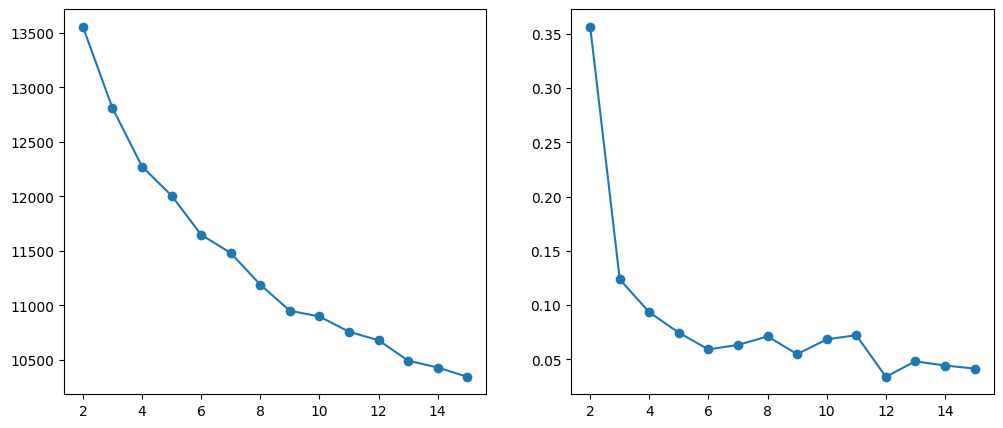
\includegraphics[width=0.8\textwidth]{selection_k_plots_Victor.png}
  \caption{Courbes WCSS et silhouette pour la sélection de $k$ (Victor)}
\end{figure}

\textbf{Mapping cluster $\rightarrow$ label (vote majoritaire)~:} pour nommer chaque cluster, on identifie la classe réelle dominante parmi ses membres. En cas de conflit, le cluster de plus haute pureté conserve l'étiquette (stratégie gloutonne).

\begin{figure}[H]
  \centering
  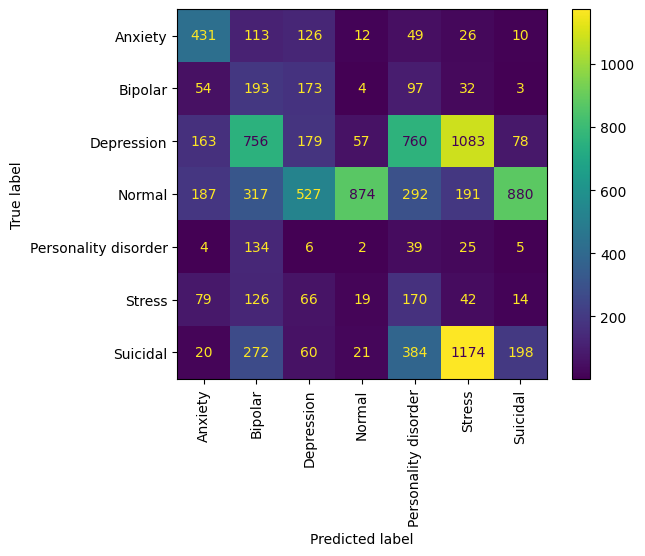
\includegraphics[width=0.8\textwidth]{mapping_results_Victor.png}
  \caption{Résultat du mapping et pureté des clusters (Victor)}
\end{figure}

\begin{remarque}
Victor a corrigé une erreur du template qui tentait de mélanger TF-IDF et Word2Vec dans la cellule de déploiement final, ce qui rendait le pipeline incohérent.
\end{remarque}

% ------------------------------------------------------------------------------
\subsubsection{Emin --- Comparaison TF-IDF et robustesse du pipeline}
% ------------------------------------------------------------------------------

Emin a complété l'étude en implémentant le pipeline complet sous \textbf{TF-IDF + SVD} pour comparer les deux représentations.

\textbf{Pourquoi utiliser SVD avec tf-IDF ?}
Le possible problème que l'on peut avoir ici est que les vecteurs TF-IDF sont très creux (beaucoup de zéros) et en très haute dimension (50\,000 features). 
Cela peut rendre la tâche de clustering plus difficile pour K-Means, qui fonctionne mieux dans des espaces denses et de dimension modérée. 
En appliquant une réduction de dimensionnalité via SVD (\textit{TruncatedSVD} sous python), on peut compacter l'information essentielle dans un espace plus petit 
(ex.~: 100 dimensions), ce qui facilite le travail de K-Means.


\begin{figure}[H]
  \centering
  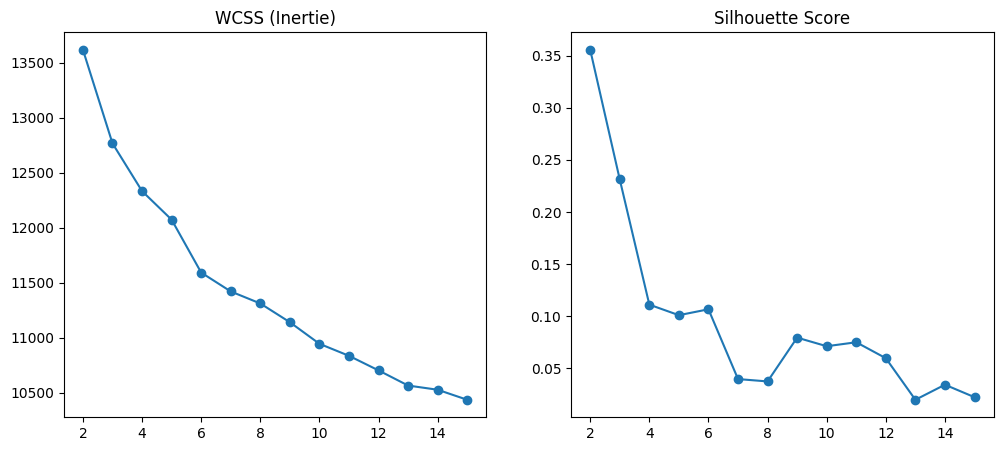
\includegraphics[width=0.8\textwidth]{selection_k_plots_Emin.png}
  \caption{Courbes WCSS et silhouette pour la sélection de $k$ (Emin)}
\end{figure}

\begin{figure}[H]
  \centering
  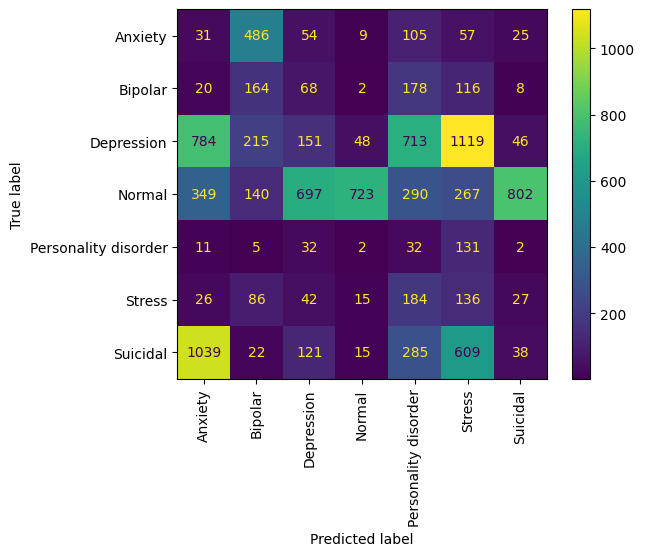
\includegraphics[width=0.8\textwidth]{mapping_results_Emin.png}
  \caption{Résultat du mapping et pureté des clusters (Emin)}
\end{figure}

Emin a également résolu des conflits de versions entre \texttt{gensim} et \texttt{scipy} dans l'environnement de travail, et standardisé la cellule de déploiement B.6 pour utiliser le modèle TF-IDF.

% ------------------------------------------------------------------------------
\subsubsection{Synthèse --- Comparaison TF-IDF vs Word2Vec pour K-Means}
% ------------------------------------------------------------------------------

\begin{center}
\renewcommand{\arraystretch}{1.2}
\begin{tabular}{lcc}
\toprule
\textbf{Critère} & \textbf{K-Means + TF-IDF} & \textbf{K-Means + Word2Vec} \\
\midrule
Meilleur $k$ retenu     & 7          & 7 \\
\textbf{Accuracy test}  & \textbf{0.4636} & 0.20 \\
Purity globale          & \textbf{0.54}   & 0.51 \\
ARI                     & \textbf{0.25}   & 0.13 \\
Besoin de SVD ?         & Oui        & Non \\
Dimension de l'espace   & 100 (après SVD) & 100 (natif) \\
Pureté max cluster      & 0.85 (\textit{Depression}) & 0.90 (\textit{Normal}) \\
Pureté min cluster      & 0.30 (\textit{Personality disorder}) & 0.30 (\textit{Bipolar}) \\
\bottomrule
\end{tabular}
\end{center}

\begin{figure}[H]
  \centering
  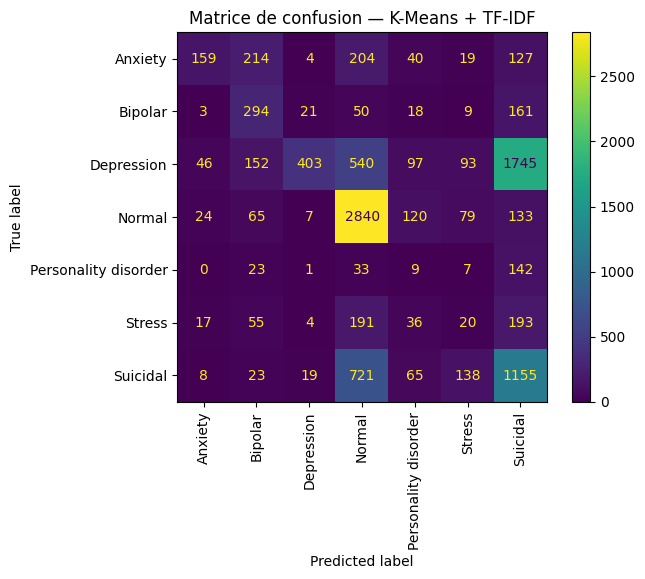
\includegraphics[width=0.8\textwidth]{matriceConfusion_Kmeans_W2V_TF_IDF_Victor.png}
  \caption{Matrice de confusion --- K-Means final (TF-IDF vs Word2Vec)}
\end{figure}

\pagebreak
\begin{remarque}
Contra-intuitivement, TF-IDF (46\,\%) surpasse Word2Vec (20\,\%). Les catégories cliniques du dataset (\textit{Depression}, \textit{Anxiety}, etc.) se reconnaissent avant tout par un \textbf{vocabulaire symptomatique spécifique}, ce que TF-IDF met précisément en avant. Word2Vec, qui regroupe les mots par contexte sémantique large, tend à fusionner \textit{Depression} et \textit{Suicidal} dans les mêmes clusters --- le mapping glouton force alors ces gros clusters sur des labels minoritaires, effondrant l'accuracy globale.
\end{remarque}

\textbf{Modèle retenu pour le non-supervisé~:} K-Means + TF-IDF.\\
\textbf{Fichier produit~:} \texttt{train\_with\_sentiments\_kmeans.csv}.

\pagebreak

% ==============================================================================
\section{Comparaison globale : supervisé vs. non-supervisé}
% ==============================================================================

\begin{center}
\renewcommand{\arraystretch}{1.2}
\begin{tabular}{lcc}
\toprule
\textbf{Critère} & \textbf{NB TF-IDF } & \textbf{K-Means TF-IDF} \\
                 & \textbf{(supervisé)} & \textbf{(non-supervisé)} \\
\midrule
\textbf{Accuracy test}          & \textbf{0.6875} & 0.4636 \\
Macro avg F1                    & 0.62            & ---    \\
Weighted avg F1                 & 0.69            & ---    \\
Voit les labels                 &                 &    \\
à l'entraînement ?              & Oui             & Non    \\
Hyperparamètre clé              & alpha = 0.05    & $k = 7$ \\
Fichier annoté                  & \texttt{train\_with\_sentiments.csv} & \texttt{train\_with\_sentiments\_kmeans.csv} \\
\bottomrule
\end{tabular}
\end{center}

L'écart de \textbf{+22 points d'accuracy} en faveur du supervisé est cohérent et attendu~: le supervisé a accès aux vrais labels pendant l'entraînement, le non-supervisé pas. Les deux méthodes utilisent la même représentation TF-IDF, donc l'écart reflète purement la différence supervisé/non-supervisé.

Les mêmes classes sont difficiles pour les deux approches (\textit{Personality disorder}, \textit{Stress}, confusion \textit{Depression}/\textit{Suicidal}). Cela pointe vers une \textbf{limite des données elles-mêmes} (classes sous-représentées, vocabulaire qui se chevauche) plutôt qu'un problème algorithmique.

\pagebreak

% ==============================================================================
\section{Décision finale : modèle transmis au Groupe 2}
% ==============================================================================

\begin{center}
\Large $\rightarrow$ \textbf{Modèle retenu : LogisticRegression + TF-IDF}
\end{center}

\begin{center}
\renewcommand{\arraystretch}{1.2}
\begin{tabular}{ll}
\toprule
\textbf{Critère} & \textbf{Justification} \\
\midrule
Accuracy 75,32\,\% & Meilleure performance absolue parmi tous les modèles testés \\
Annotations fiables & Les labels transmis au Groupe 2 doivent être les plus corrects \\
                    & possible pour que le filtrage par sentiments soit utile \\
Modèle léger        & LR est rapide à déployer et à sérialiser (\texttt{.pkl}) \\
\bottomrule
\end{tabular}
\end{center}

\textbf{Fichier à transmettre au Groupe 2~:} \texttt{train\_with\_sentiments.csv}\\
\textbf{Colonne d'annotation~:} \texttt{predicted\_sentiment}\\
\textbf{Classes prédites~:} \texttt{Anxiety}, \texttt{Bipolar}, \texttt{Depression}, \texttt{Normal}, \texttt{Personality disorder}, \texttt{Stress}, \texttt{Suicidal}

\begin{avertissement}
\textbf{Note pour le Groupe 2~:} Il existe toujours une confusion importante entre 
les classes \textit{Depression} et \textit{Suicidal} (529 vrais \textit{Suicidal} 
prédits \textit{Depression}), ce qui peut biaiser les analyses de sentiments. 
Il est recommandé de traiter ces deux classes avec prudence, 
voire de les regrouper en une seule catégorie «~At Risk~» pour les besoins 
du filtrage par sentiments.

\end{avertissement}

% ==============================================================================
\section{Points de vigilance et perspectives}
% ==============================================================================

\begin{itemize}
  \item \textbf{Déséquilibre des classes~:} \textit{Depression} est sur-représentée dans \\
  \texttt{combined\_data.csv}, ce qui biaise tous les modèles. Une solution (non implémentée faute de temps) serait le sur-échantillonnage SMOTE ou l'ajustement de \texttt{class\_weight}.

  \item \textbf{Confusion \textit{Depression} / \textit{Suicidal}~:} problème critique dans le contexte médical. La LR avec régularisation L1 (\texttt{penalty='l1'}, \texttt{solver='saga'}) améliore ce point mais le temps d'entraînement est prohibitif ($\approx 4$\,h). À envisager si plus de ressources de calcul sont disponibles.

  \item \textbf{R² non pertinent~:} cette métrique ne doit pas être utilisée pour évaluer des classifieurs multi-classes à labels nominaux. L'accuracy, le F1-score et la matrice de confusion sont les indicateurs à retenir.

  \item \textbf{Amélioration possible~:} la Logistic Regression de Logan (LR + TF-IDF, \\
  \texttt{class\_weight='balanced'}) est prometteuse --- accuracy de 75.32\,\% et gains de $+0.20$ à $+0.26$ de F1 sur les classes minoritaires --- et devrait être envisagée comme version finale si le temps de calcul le permet.
\end{itemize}

\end{document}